\documentclass[12pt]{beamer}
\usepackage{../latex-sty/mypres}
\usepackage[utf8]{inputenc}
\usepackage[T2A]{fontenc}
\usepackage[russian]{babel}

\expandafter\def\expandafter\insertshorttitle\expandafter{%
  \insertshorttitle\hfill%
  \insertframenumber\,/\,\inserttotalframenumber}
\title[Семинар 8]{Методы оптимизации. \\
 Семинар 8. Сопряжённые функции}
\author{Александр Катруца}
\institute{Московский физико-технический институт,\\
Факультет Управления и Прикладной Математики} 
\date{\today}

\begin{document}
\begin{frame}
\maketitle
\end{frame}

\begin{frame}{Напоминание}
\begin{itemize}
\item Субградиент и субдифференциал
\item Условный субдифференциал
\item Способы вычисления субдифференциалов
\end{itemize}
\end{frame}

\begin{frame}{Определение}
\begin{block}{Снова сопряжённое?}
\begin{itemize}
\item Ранее были рассмотрены сопряжённые (двойственные) множества и, в частности, конусы
\item Сейчас будут рассмотрены сопряжённые (двойственные) функции
\item Далее будет введена двойственная оптимизационная задача 
\end{itemize}
\end{block}

\begin{block}{Определение}
Пусть $f: \bbR^n \rightarrow \bbR$. 
Функция $f^*: \bbR^n \rightarrow \bbR$ называется сопряжённой функцией к функции $f$ и определена как
\vspace{-4mm}
\[
f^*(\by) = \sup\limits_{\bx \in dom \; f} (\by^{\T}\bx - f(\bx)).
\vspace{-3mm}
\]
Область определения $f^*$~--- это множество таких $\by$, что супремум конечен. 

\end{block}
\end{frame}

\begin{frame}{Свойства}
\begin{itemize}
\item Сопряжённая функция $f^*$ всегда выпукла как супремум линейных функций независимо от выпуклости $f$
\item Неравенство Юнга-Фенхеля: $\by^{\T}\bx \leq f(\bx) + f^*(\by)$

Обобщение квадратичного случая: $\by^{\T}\bx \leq \frac{1}{2}\bx^{\T}\bx + \frac{1}{2}\by^{\T}\by$
\item Если $f$~--- дифференцируема, то $f^*(\by) = \nabla f^{\T}(\bx^*)\bx^* - f(\bx^*)$, где $\bx^*$ даёт супремум.
\item Если $f$ выпукла и замкнута, то $f^{**} = f$
\end{itemize}
\end{frame}

\begin{frame}{Геометрический смысл}
\begin{figure}
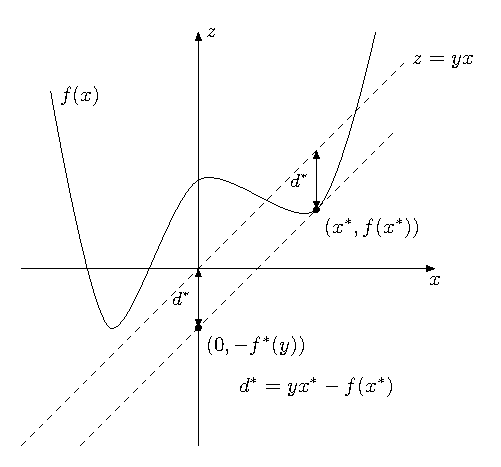
\includegraphics[scale=1]{geom.pdf}
\end{figure}
\end{frame}

\begin{frame}{Примеры}
\begin{enumerate}
\item Линейная функция: $f(\bx) = \ba^{\T}\bx + b$
\item Отрицательная энтропия: $f(x) = x\log x$
\item Индикаторная функция множества $S$: $I_S(x) = 0$ iff $x \in S$
\item Норма: $f(\bx) = \|\bx\|$.
\item Квадрат нормы: $f(\bx) = \frac{1}{2}\|\bx\|^2$
\end{enumerate}
\end{frame}

\begin{frame}{Операции с сопряжёнными функциями}

\begin{itemize}
\item Разделение переменных: $f(x_1, x_2) = g(x_1) + h(x_2)$ и $f^*(y_1, y_2) = g^*(y_1) + h^*(y_2)$
\item Сдвиг аргумента: $f(\bx) = g(\bx - \ba)$ и $f^*(\by) = \ba^{\T}\by + g^*(\by)$
\item Суперпозиция с обратимым линейным преобразованием: $f(\bx) = g(\bA\bx)$ и $f^*(\by) = g^*(\bA^{-\T}\by)$
\item Инфимальная конволюция (свёртка инфимумом):  $f(x) = (h \square g)(x) = \inf\limits_{u + v = x} (h(u) + g(v))$ и $f^*(y) = h^*(y) + g^*(y)$
\end{itemize}

\end{frame}

\begin{frame}{Moreau-Yosida envelope}
\begin{itemize}
\item $f(\bx)$ выпуклая, но \emph{негладкая}
\item Moreau-Yosida envelope ($\lambda > 0$)
\[
M_{\lambda f}(\bx) = \inf\limits_{\bu} (f(\bu) + \frac{1}{2\lambda}\|\bx - \bu\|^2_2) = \left(f \square \frac{1}{2\lambda} \|\cdot\|_2^2\right)(\bx)
\]
\item Функция Хьюбера~-- $M_{\lambda f}$ для модуля
\begin{itemize}
\item $f(x) = |x|$
\item $M_{\lambda f}(x) = 
\begin{cases}
\frac{x^2}{2\lambda} & |x| \leq \lambda\\
|x| - \lambda / 2 & |x| \geq \lambda
\end{cases}$
\end{itemize}
\begin{block}{Упражнение}
\begin{itemize}
\item Нарисуйте на одном графике $f(x)$ и $M_{\lambda f}(x)$
\item Получите выражение $M_{\lambda f}$ для $f(\bx) = \|\bx\|_1$ 
\end{itemize}
\end{block}
\end{itemize}

\end{frame}

\begin{frame}{Почему получилась гладкая функция?}
\begin{itemize}
\item $M_{\lambda f}(\bx)$~-- выпукла
\item $M^*_{\lambda f}(\by) = f^*(\by) + \frac{\lambda}{2}\|\by\|_2^2$~-- сильно выпукла с параметром $\lambda$
\item $M_{\lambda f} = M^{**}_{\lambda f} = (f^* + \frac{\lambda}{2}\|\cdot \|_2^2)^*$
\item Сопряжённая функция к сильно выпуклой функции является гладкой $\Rightarrow M_{\lambda f}$~-- гладкая функция и 
\[
M'_{\lambda f}(\bx) = \frac{1}{\lambda} (\bx - \bu^*), \quad \bu^* = \argmin_{\bu} \left(f(\bu) + \frac{1}{2\lambda}\|\bx - \bu\|^2_2\right) 
\]
\end{itemize}

\begin{block}{Важное свойство}
Множество точек минимума $f$ и $M_{\lambda f}$ совпадает.
\end{block}

\end{frame}

\begin{frame}{Резюме}

\begin{itemize}
\item Сопряжённые функции
\item Неравенство Юнга-Фенхеля и другие свойства
\item Сглаживание негладких функций
\item Примеры
\end{itemize}

\end{frame}

\end{document}